\documentclass[expanded]{lkx_pset}

\title{Math 213b Problem Set 10}
\author{Lev Kruglyak}
\due{April 17, 2024}

\usepackage{graphicx}

\newcommand{\D}{\mathbb{D}}
\newcommand{\x}{\mathbf{x}}
\usepackage{pgfplots}
\pgfplotsset{
	compat=1.12,
}


\collaborator{AJ LaMotta}
\collaborator{Jarell Cheong}

\begin{document}
\maketitle

\begin{problem}{1}
If $X$ is a manifold and $p_{0}\in X$ is a base-point, then the universal cover $\widetilde X$ can be defined as the set of pairs $(p, [\gamma])$ consisting of a point $p\in X$ and a homotopy class of paths $\gamma$ from $p_{0}$ to $p$.
\end{problem}
\begin{parts}
	\begin{part}{}
		Let $X$ be a compact connected Riemann surface of genus $3$, and let
		$\alpha_{1}$, $\alpha_{2}$, $\alpha_{3}$ be a basis for the
		holomorphic differentials on $X$. Let $p_{0}$ be a basepoint and
		let $U\subset X$ be a neighborhood of $p_{0}$ homeomorphic to a disk.
		Define
		\[
			\definefunction{F}{\widetilde{U}}{\C^3}{p}{ \int_{p_{0}}^{p} \alpha_{1}, \int_{p_{0}}^{p} \alpha_{2},  \int_{p_{0}}^{p} \alpha_{3}}
		\]
		where the path of integration is chosen to lie always in $U$.
		Assuming that $p_{0}$ is not a Weierstrass point, show that
		$F(a)+F(b)+F(c) =0$ only if $a=b=c=p_{0}$ in $U$.
	\end{part}

	Let's begin with the forward direction, so suppose that $F(a)+F(b)+F(c)=0$. This means that
	\[
		\int_{p_0}^a\alpha_i + \int_{p_0}^b\alpha_i + \int_{p_0}^c \alpha_i = 0\quad\textrm{for}\quad i\in \{1,2,3\}.
	\]
	However, we know that $\alpha_1,\alpha_2,\alpha_3$ form a basis for $H^{1,0}(X)$, it follows by linearity that
	\[
		\int_{p_0}^a \alpha + \int_{p_0}^b\alpha + \int_{p_0}^c \alpha = 0\quad\textrm{ for all}\quad \alpha\in H^{1,0}(X).
	\]
	Thus, by Abel's theorem, $a+b+c-3p_0$ is a principal divisor on $X$, and so there must exist some $f\in \mathcal{M}_X$ such that
	\[
		a+ b+c-3p_0 = \div(f).
	\]
	Since $p_0$ is not a Weierstrass point, $f$ cannot have just a pole of order at most $3$ and no other poles, so it follows that $a=b=c=p_0$.
\end{parts}

\begin{problem}{2}
Show that
\begin{align*}
	\int_0^1 \frac{dx}{\sqrt{x(x-1)(x-3)}}
	 & \int_1^3 \frac{x dx}{\sqrt{-x(x-1)(x-3)}} = \\
	 & \int_1^3 \frac{dx}{\sqrt{-x(x-1)(x-3)}}
	\int_0^1 \frac{x dx}{\sqrt{x(x-1)(x-3)}} + 2\pi.
\end{align*}

Note that all the expressions inside the square roots are real,
non-negative functions on the given intervals of integration;
so all four integrals are to be interpreted as real integrals.
\end{problem}

By a similar argument to a problem on the previous problem set, we can define $X', X, \pi, \widetilde{\pi}$. Then we can get $R_{\widetilde{\pi}}=4$, $g_X=1$, and $\infty$ is now ramified over $X$ with preimage $\infty$. Then the forms $\alpha = dx/y$ and $\alpha'=x\,dx/y$ are holomorphic away from $\infty$.

Next, we'll prove that $\alpha$ is of the first kind. Notice that in coordinates $z=1/\sqrt{x}$, we have
\[
	\alpha = \frac{-2\,dz}{\sqrt{1-4z^2+3z^4}}.
\]
If we plug in $z=0$, we see that $\alpha$ is holomorphic at $x=\infty$, and so is of the first kind. Similarly, we see that
\[
	\alpha' = \frac{-2\,dz}{z^2\sqrt{1-4z^2+3z^4}} = \left(-\frac{2}{z^2}-4-9z^2+O(z^4)\right)\,dz\quad\textrm{at } z=0,
\]
and so $\alpha'$ is of the second kind. By the Riemann bilinear relations for differentials of the second kind, we see that
\[
	\int_a \alpha' \int_b \alpha - \int_b \alpha' \int_a \alpha = 2\pi i\,\textrm{Res}_\infty(f\alpha)
\]
where $f$ is the integral of $\alpha'$, and $a$ and $b$ are the red and blue loops in the following picture of a relevant portion of $X'$ intersected with the real $x$-axis below:

\begin{center}
	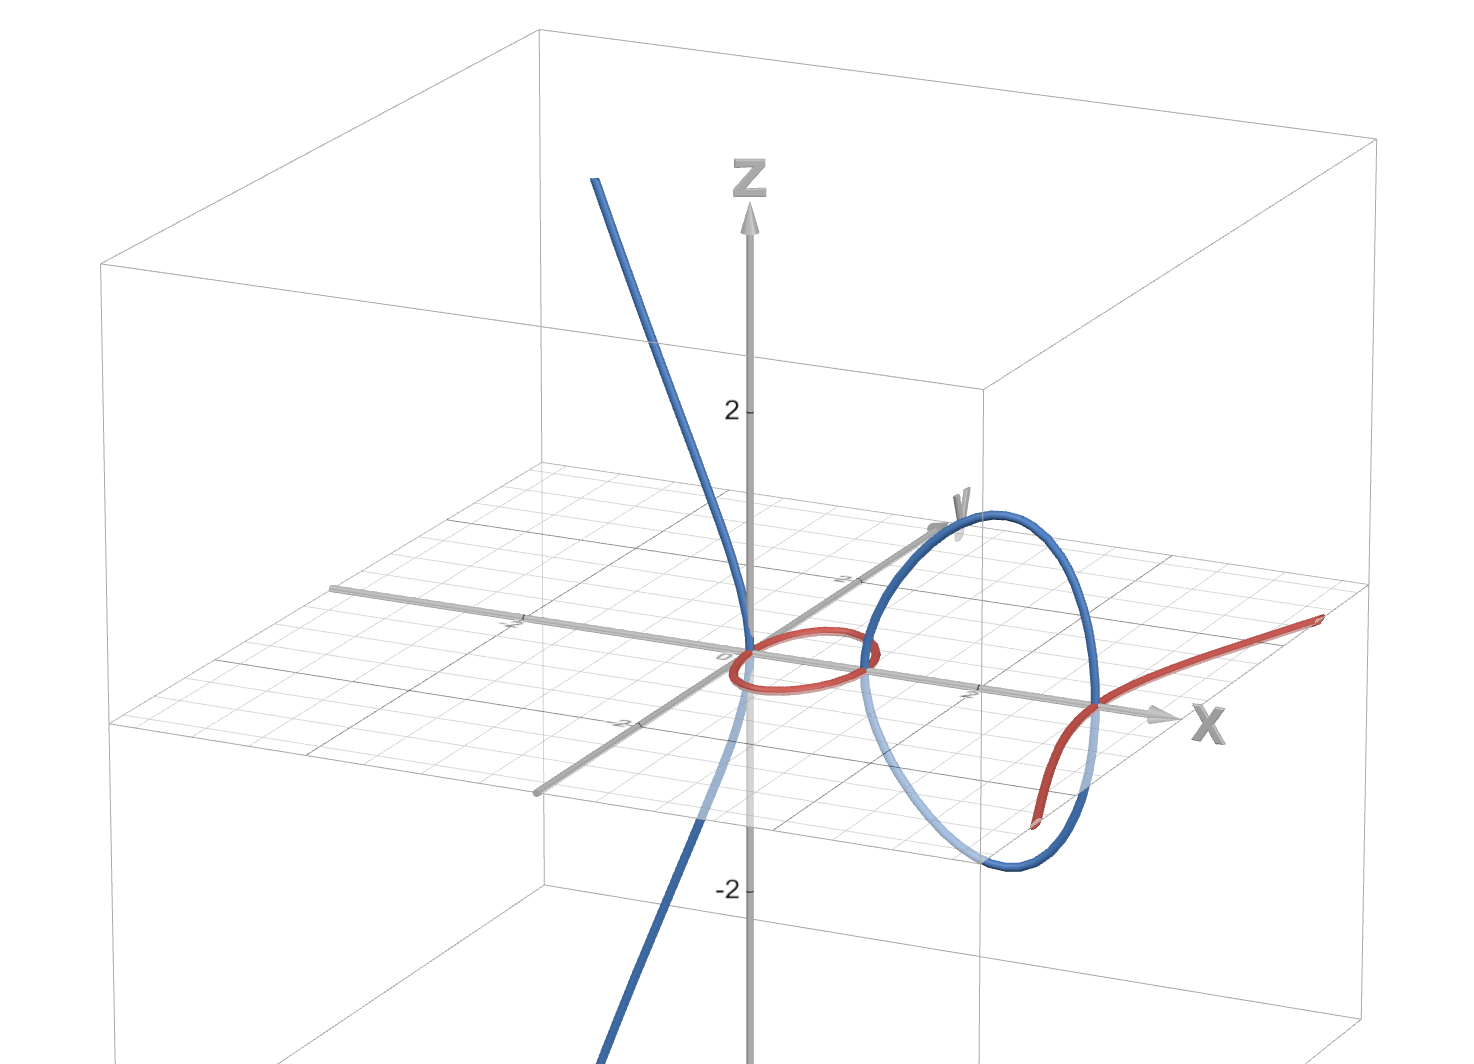
\includegraphics[scale=0.5]{10.2.png}

	(\emph{Credit to Jarell Cheong for producing the diagram.})
\end{center}

Now near $z=0$, we have $\alpha' = -2/z^2+O(1)$, so $f=2/z+O(z)$ and
\[
	f\alpha = \left(-\frac{4}{z}+ O(1)\right)\,dz \quad\implies\quad \textrm{Res}_\infty(f\alpha)=-4.
\]

Now let's parametrize $a$ by
\[
	a(x) = \begin{cases} (x, \sqrt{x(x-1)(x-3)}) & x=1\textrm{ to } x=0,\\ (x,-\sqrt{x(x-1)(x-3)})& x=0\textrm{ to }x=1.\end{cases}
\]
Similarly, we parametrize $b$ by
\[
	b(x) = \begin{cases} (x, -\sqrt{-x(x-1)(x-3)}) & x=1\textrm{ to } x=3,\\ (x,-i\sqrt{-x(x-1)(x-3)})& x=3\textrm{ to }x=1.\end{cases}
\]
Now, after dividing by the residue of $-4$, the bilinear relation becomes
\begin{align*}
	\int_0^1 \frac{dx}{\sqrt{x(x-1)(x-3)}}
	 & \int_1^3 \frac{x dx}{i\sqrt{-x(x-1)(x-3)}} = \\
	 & \int_1^3 \frac{dx}{i\sqrt{-x(x-1)(x-3)}}
	\int_0^1 \frac{x dx}{\sqrt{x(x-1)(x-3)}} + 2\pi.
\end{align*}
Multiplying by $i$, we get our desired equality.

\begin{problem}{3}
Let $X$ be a compact, connected Riemann surface of genus $g$, and let $a_i$, $b_i$
be standard set of curves on $X$. In the traditional terminology,
a differential
$\eta$ is said to be of the \emph{first kind} if it is holomorphic.
It is said to be of the \emph{second kind} if it is meromorphic but
has zero residues at all its poles.  A general meromorphic
differential is said to be of the \emph{third kind}.  A differential
is \emph{normalized} (with respect to the chosen $a$ and $b$ curves)
if all its $A$-periods are zero.
\end{problem}

\begin{parts}
	\begin{part}{}
		Show that every meromorphic differential $\eta$ has a unique
		decomposition,
		\[
			\eta = \eta_1 + \eta_2 +\eta_3,
		\]
		where $\eta_1$ is of the first kind, $\eta_2$ is a normalized
		differential of the second kind, and $\eta_3$ is a normalized
		differential of the third kind having only \emph{simple} poles.
	\end{part}

	Let's suppose $\eta$ has principal parts
	\[
		P_i\,dz_i = a_{i,-1} z_i^{-1} + \cdots + a_{i,-k}z_i^{-k}\,dz_i.
	\]
	Sine a meromorphic differential with prescribed principal parts exists if and only if the sum of their residues is zero, there exists a meromorphic differential with prescribed principal parts \[Q_i \,dz_i = a_{i,-2}z_i^{-2}+\cdots + a_{i,-k}z_i^{-k}\,dz_i.\] Let's call this meromorphic differential $\beta_2$, and it's clear to see that it is of the second kind. Next, consider the meromorphic differential with prescribed principal parts \[R_i\,dz_i = a_{i,-1}z_i^{-1}\,dz_i,\] which we'll call $\beta_3$. This has only simple poles, and so $\beta_3$ is of the third kind.

	Finally, let $\omega_i$ be a normalized basis for $H^{1,0}(X)$, and define the terms
	\[
		\lambda_{j,2} = -\int_{a_j} \beta_2, \quad \lambda_{j,3} = -\int_{a_j}\beta3,\quad\implies\quad \alpha_2 = \sum_j \lambda_{j,2}\omega_j,\quad\alpha_3=\sum_j\lambda_{j,3}\omega_j.
	\]
	Notice that $\eta_2 = \alpha_2 + \beta_2$ and $\eta_3 = \alpha_3 + \beta_3$ are normalized by construction, and also of second and third kinds respectively. Then, the form $\eta_1 = \eta - \eta_2 - \eta_3$ is a holomorphic form because $P_i dz_i - Q_i\,dz_i - R_i\,dz_i=0$. This proves the existence of the decomposition.

	To prove uniqueness, we suppose that $\eta_1+\eta_2+\eta_3 = \eta'_1 + \eta'_2 + \eta'_3$. We know that $\eta_3$ and $\eta'_3$ must be equal since they have the same polar parts, meaning their difference is a holomorphic differential whose $A$-periods. By a similar argument, we get $\eta_2=\eta'_2$ and $\eta_1=\eta'_1$.

	\begin{part}{}
		Let $D$ be a divisor $2p + 2q$ on $X$. (The points
		$p$ and $q$ are distinct.) Let $V$ be
		the vector space of meromorphic differentials $\eta$ with
		$\mathrm{div}(\eta) + D \ge 0$.  Using the above decomposition, we
		can write
		\[
			V = V_1 \oplus V_2 \oplus V_3.
		\]
		What are the dimensions of $V_1$, $V_2$ and $V_3$?
	\end{part}

	By the Riemann-Roch theorem, we get
	\[
		\dim V_1 \oplus V_2\oplus V_3 = \dim V = \dim \Omega(D) = g+3,
	\]
	since $\deg(-D)=-4$ so $\ell(-D)=0$. Since $V_1\oplus V_3=\Omega(p+q)$, it follows that $\dim V_1 \oplus V_3 = g+1$, and since $D\geq 0$, it follows that $V_1=H^{1,0}(X)$ and so $\dim V_1 = \dim H^{1,0}(X)=g$. This means that
	\[
		\begin{aligned}
			\dim V_1 & = g, \\
			\dim V_2 & =2,  \\
			\dim V_3 & = 1.
		\end{aligned}
	\]
\end{parts}

\end{document}
